\documentclass[a4paper]{report}

\usepackage{graphicx}
\graphicspath{{./images/} }


\title{Vaja 31 Torzijsko nihalo}
\author {Jure Kos}
\date {5.1.2022}

\begin{document}
\maketitle

\chapter*{Uvod}

S pomočjo vsiljenega nihanja smo poskušali narisati resonančno krivuljo torzijskega nihala. Nihalo je bilo v vaji nedušeno, delno dušeno in nato zelo dušeno. Dušili smo ga z magnetom.
Prav tako nas je zanimal fazni premik, ki nastane pri vsiljenem nihanju ter povprečna sprejeta moč.

\section*{Naloga}
Izmeri in izračunaj resonančno krivuljo za torzijsko nihalo pri dveh različnih dušenjih.

\section*{Pripomočki}

1. Torzijsko nihalo,\\
2. elektromotor z vzvodom,\\
3. štoparica.\\




\chapter*{Navodila}

Nedušeno nihalo s prstom poženi, da začne nihati in izmeri nihajni čas 5 nihajev. Istočasno odberi prvo in zadnjo amplitudo na isti strani. S tem lahko izračunaš koeficient dušenja $\beta$ ter lastno frekvenco $ \omega_0$, ki bi jo imelo nedušeno nihalo. 
 Pred merjenjem se sprehodi s potenciometrom čez frekvence, da dobiš približno predstavo resonačne krivulje. Po tem daj potenciometer na najmanjšo možno frekvenco $\omega_0$ , počakaj,
 da se nihanje umiri, ter odčitaj amplitudo $B_0$. Ponovi postopek za višje frekvence, in odčitaj amplitudo $B$ vedno na isti strani. Gosteje izvajaj meritve okrog resonance. Isto ponovi za delno dušeno in zelo dušeno nihalo.\par
\noindent Nariši:

\begin{itemize}
\item na isti graf resonančne krivulje  za nedušeno, delno dušeno in zelo dušeno, kjer je na abcisi $\omega/ \omega_0$ in na ordinati $B/B_0$
\item graf faznega premika v odvisnosti $\omega/ \omega_0$
\item graf povprečno sprejete moči v odvisnosti $\omega/\omega_0$
\end{itemize}

\noindent Določi enačbo resonančne krivulje z merjenimi $B_0$, $\omega_0$ in $\beta$.


\section*{Skica}
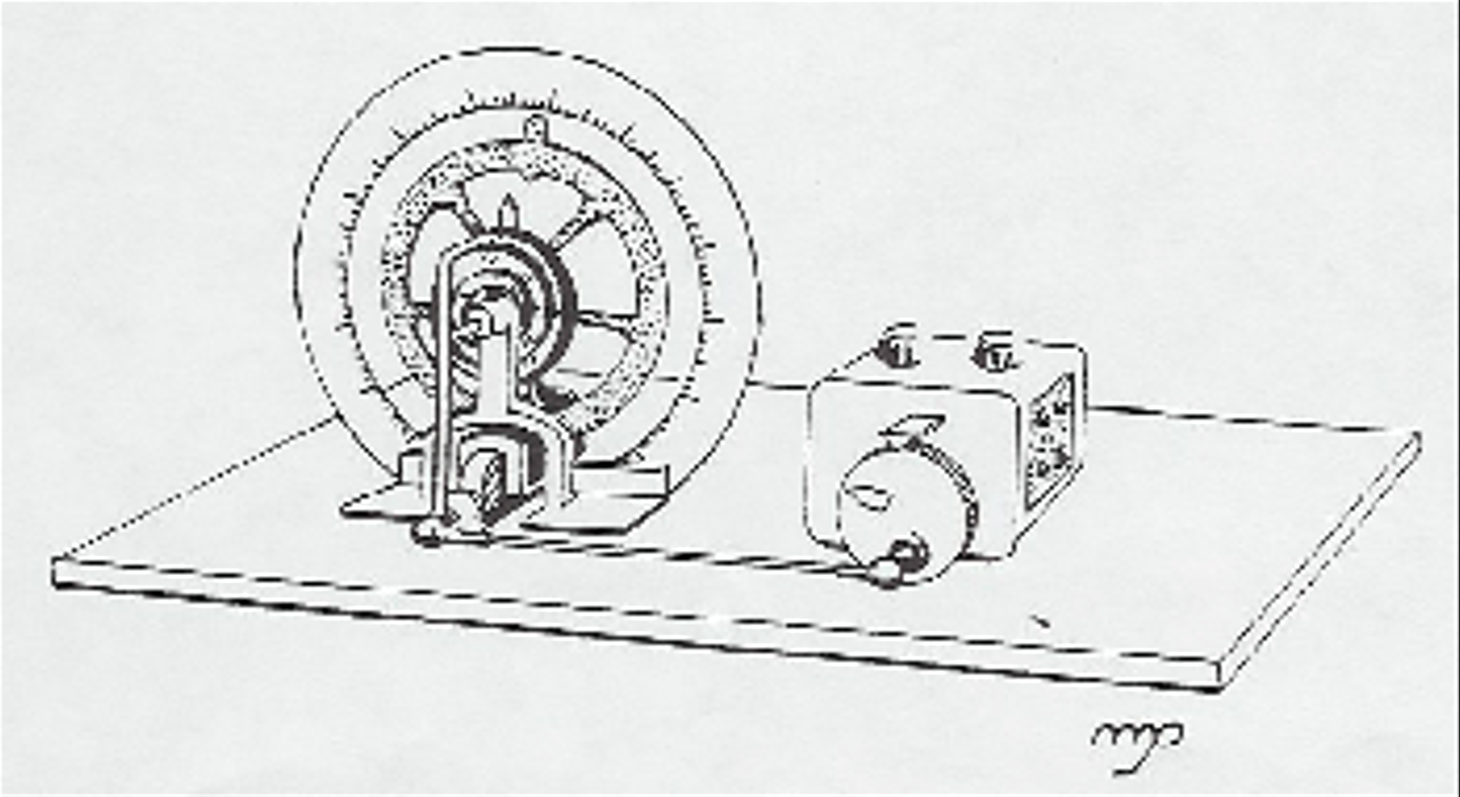
\includegraphics[width=\textwidth]{Skica}



\chapter*{Nedušeno nihanje}

Število nihajev $N = 5$\\
Nihajni čas 5 nihajev $ t = 12,11s \pm 0,05s$\\
Nihajni čas:

\[
  t_0 = \frac{t_5}{N} = \frac {12,11s}{5} = 2,42s \pm 0,01s
\]

Lastna krožna frekvenca nihala $\omega_d$:

\[
  \omega_d = \frac{2\pi}{t_0} = \frac{2\pi}{2.4s} =2,26s^{-1} \pm 0,01s^{-1}
\]

Prva amplituda $A_0 = 22 \pm 0,25$, Zadnja amplituda $A_5 = 9 \pm 0,25$\\
Koeficient dušenja $\beta$:

\[
  \beta = \frac{\omega_d}{2\pi n}\ln\frac{A_0}{A_n} = \frac{2,26s^{-1}}{2 \pi 5}\ln\frac{22}{9} =0,06s^{-1} \pm 0,01s^{-1}
\]

Lastna frekvenca $\omega_0$:

\[
  \omega_0 = \sqrt{\omega_d^2 + \beta^2} = \sqrt{(2,26s^{-1})^2 + (0,06s^{-1})^2} =2,26s^{-1} \pm 0,002s^{-1}
\]

\chapter*{Malo dušeno nihanje}

Število nihajev $N = 5$\\
Nihajni čas 5 nihajev $ t = 11,79s \pm 0,05s$\\
Nihajni čas:

\[
  t_0 = \frac{t_5}{N} = \frac {11,79s}{5} =2,36s \pm 0,004s
\]

Lastna krožna frekvenca nihala $\omega_d$:

\[
  \omega_d = \frac{2\pi}{t_0} = \frac{2\pi}{2,36s} = 2,66s^{-1} \pm 0,01s^{-1}
\]

Prva amplituda $A_0 = 22 \pm 0,25$, Zadnja amplituda $A_5 = 4 \pm 0,25$\\
Koeficient dušenja $\beta$:

\[
    \beta = \frac{\omega_d}{2\pi n}\ln\frac{A_0}{A_n} = \frac{2,36s^{-1}}{2 \pi 5}\ln\frac{22}{4} =0,13 s^{-1} \pm 0,01s^{-1}
\]

Lastna frekvenca $\omega_0$:

\[
    \omega_0 = \sqrt{\omega_d^2 + \beta^2} = \sqrt{(2,66s^{-1})^2 + (0,13s^{-1})^2} = 2,66\pm 0,003s^{-1}
\]

\chapter*{Zelo dušeno nihanje}

Število nihajev $N = 5$\\
Nihajni čas 5 nihajev $ t = 12,21s \pm 0,05$\\
Nihajni čas:

\[
  t_0 = \frac{t_5}{N} = \frac {12,21s}{5} = 2, 44s \pm 0,01s
\]

Lastna krožna frekvenca nihala $\omega_d$:

\[
  \omega_d = \frac{2\pi}{t_0} = \frac{2\pi}{2.44s} =2,58 s^{-1} \pm 0,01 s^{-1}
\]

Prva amplituda $A_0 = 22 \pm 0,25$\\
Zadnja amplituda $A_5 = 1 \pm 0,25$\\
Koeficient dušenja $\beta$:

\[
    \beta = \frac{\omega_d}{2\pi n}\ln\frac{A_0}{A_n} = \frac{2,58s^{-1}}{2 \pi 5}\ln\frac{22}{1} =0,25s^{-1} \pm 0,1s^{-1}
\]

Lastna frekvenca $\omega_0$:

\[
    \omega_0 = \sqrt{\omega_d^2 + \beta^2} = \sqrt{(2,58s^{-1})^2 + (0,25s^{-1})^2} = 2,59s^{-1} \pm 0,03s^{-1}
\]

\chapter*{Grafi}

\noindent Graf resonančne krivulje: \newline

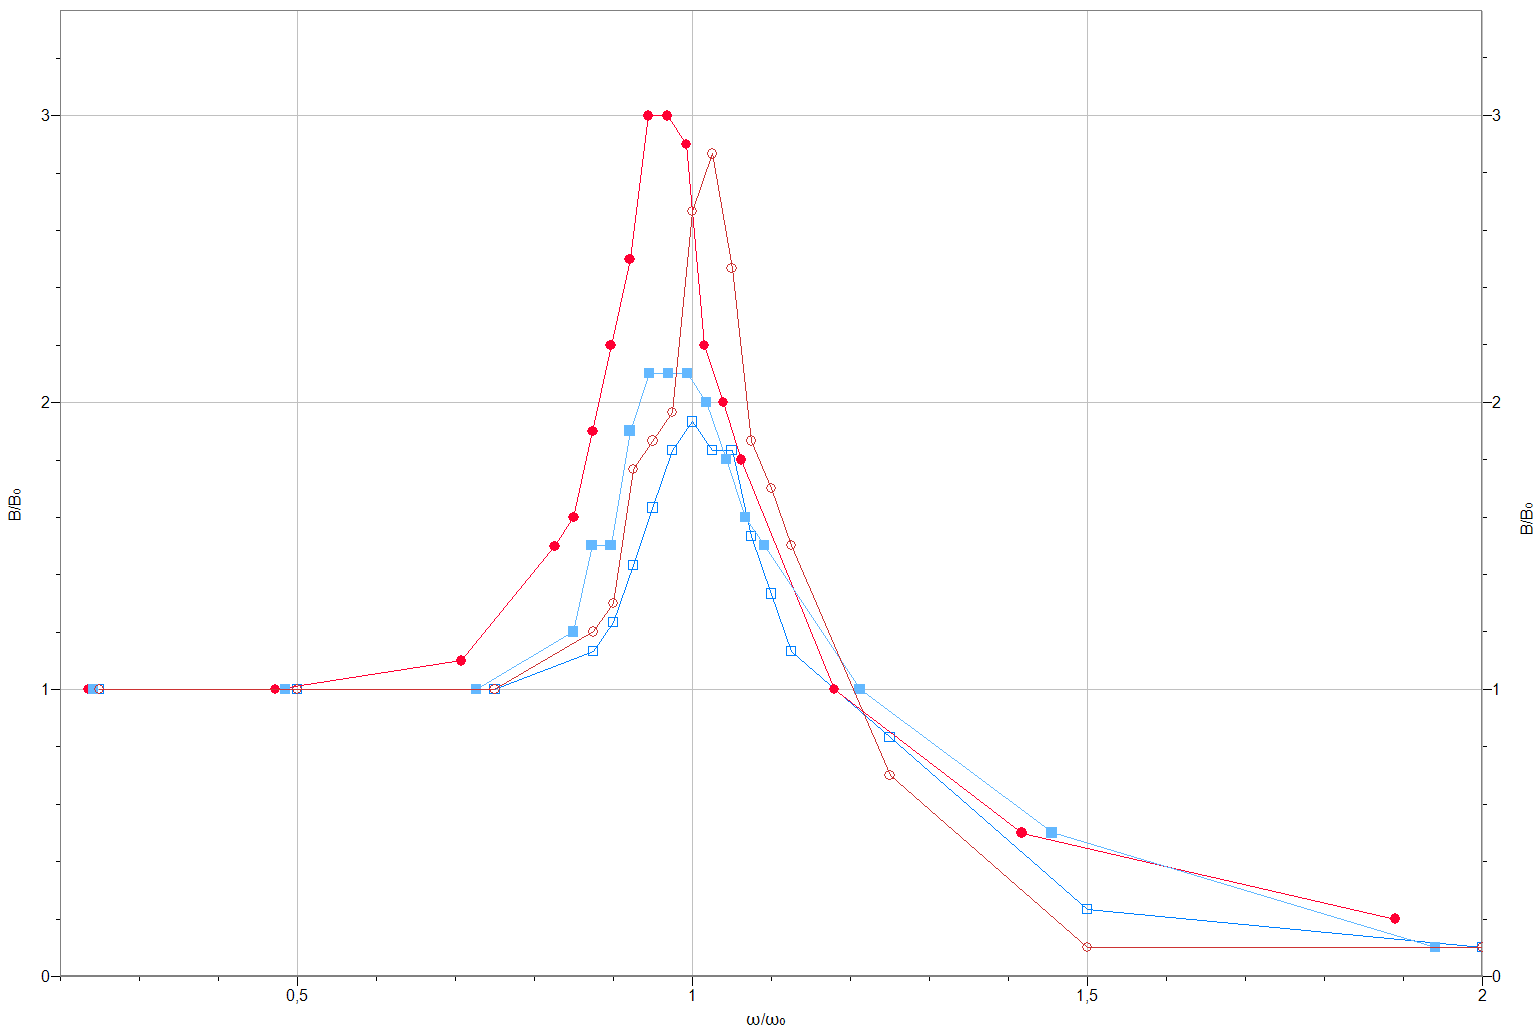
\includegraphics[width=\textwidth]{Resonanca}

\pagebreak
\noindent Graf faznega premika:\newline

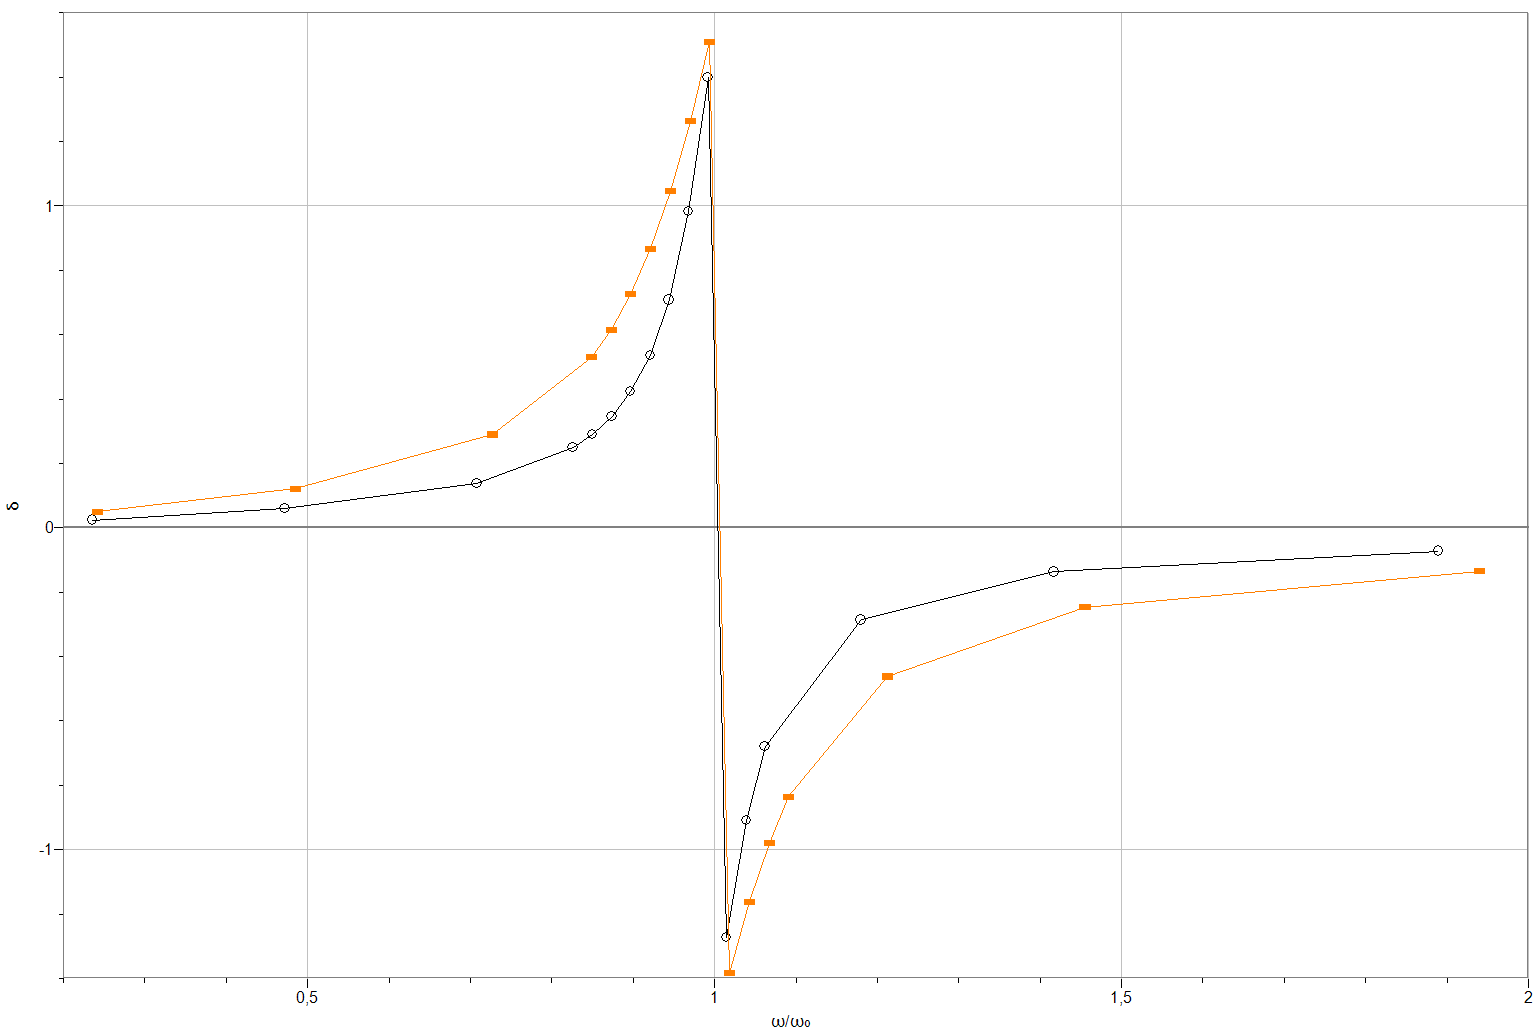
\includegraphics[width=\textwidth]{Fazni zamik}

\noindent Graf povprečno sprejete moči: \newline

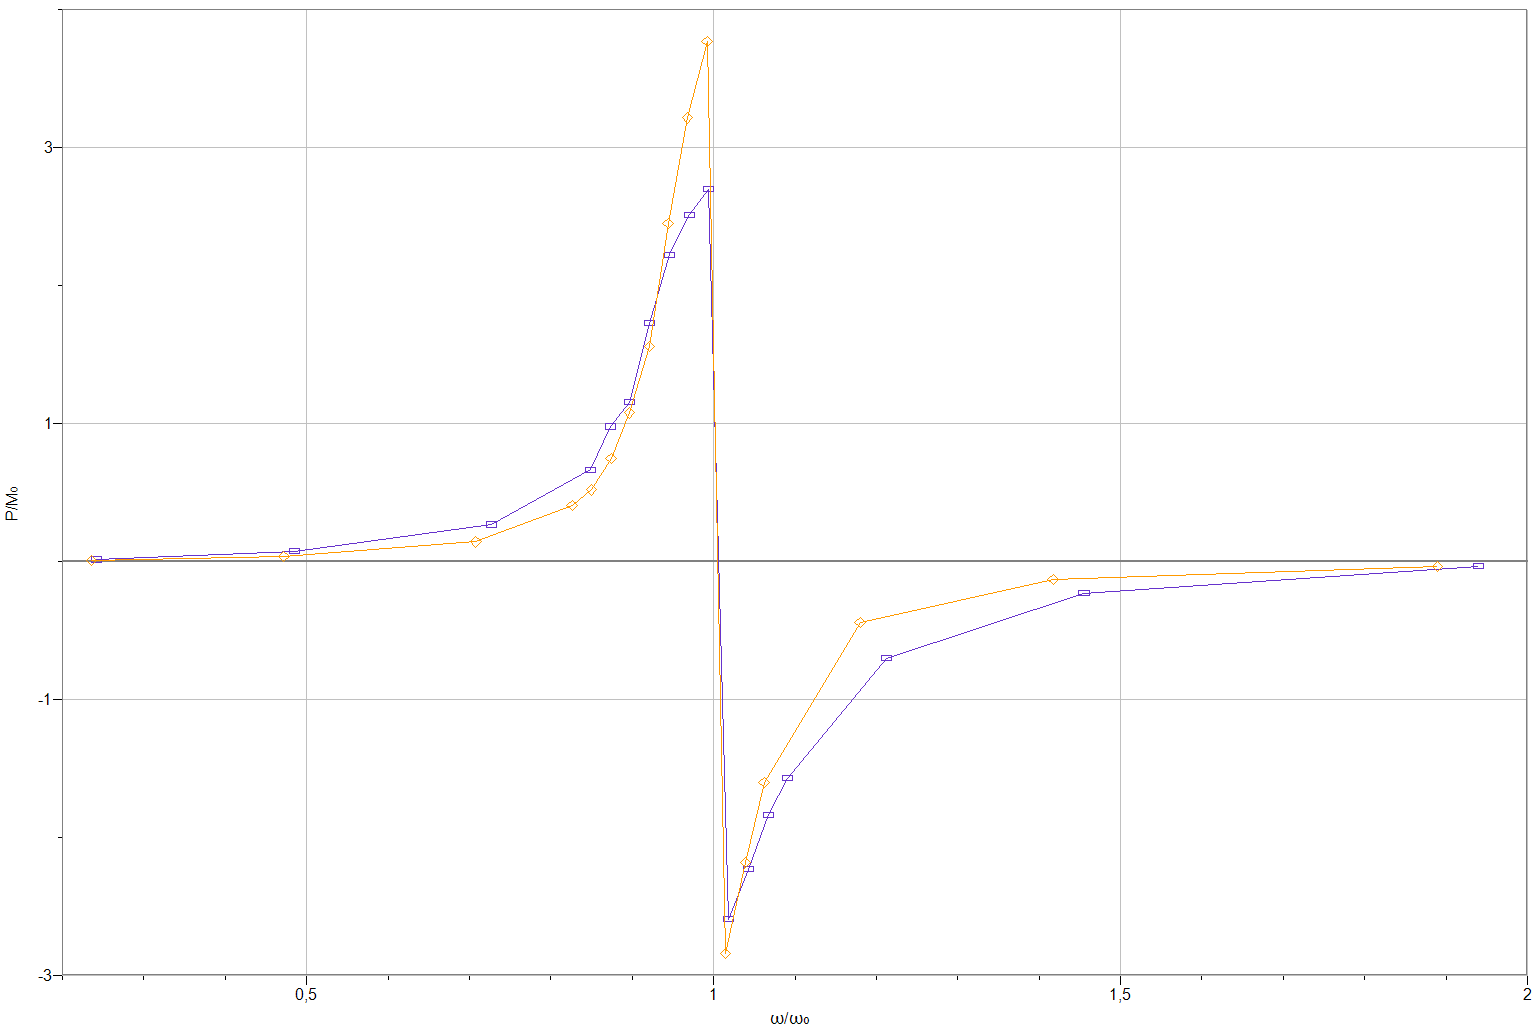
\includegraphics[width=\textwidth]{Prejeta moč}

\end{document}